\section{Pruebas y despliegue}

En esta sección vamos a unificar las pruebas y despliegue debido a la naturaleza de la aplicación. El desarrollo de esta fue articulado para los ambientes de desarrollo y ambientes productivos como una aplicación cargada sobre la nube de amazon, en forma de contenedores docker. Esto permite la transparencia del servicio respecto de la infraestructura. Para efectos de el despliegue en producción, esta fue montada sobre un ambiente en ElasticBeanstalk, en modo contenedor, pasando por medio de un balanceador de carga de segunda generación.

Debido a esto, solo existe un punto de conexión de la aplicación hacia el exterior el cual es el puerto 443 para conexiones HTTPS. Por otro lado, para la version de producción se utilizó una base de datos AWS RDS MSSQL 2017, la cual tiene accesos restringidos por medio de grupos de seguridad.

Debido a esto, no es posible replicar directamente la arquitectura para nuestros efectos, sin embargo, podemos modelar las condiciones utilizando herramientas como docker-compose para levantar un ambiente local de pruebas.

Para estos efectos, podemos utilizar la siguiente especificación para poder implementar una réplica de la infraestructura:

\begin{minted}[linenos,tabsize=2,breaklines,fontsize=\scriptsize]{yaml}
    version: "3"
    services:
      database:
        image: mcr.microsoft.com/mssql/server:2017-CU8-ubuntu
        container_name: 'database'
        environment:
          - SA_PASSWORD=Password21
          - ACCEPT_EULA=Y
        volumes: 
          - db-data:/var/opt/mssql
        ports:
          - '1433:1433'
        expose:
          - 1433
      
      base: 
        build:
          context: ./core
          dockerfile: Dockerfile
        depends_on: 
          - database
        links:
          - database
        environment:      
          # - ASPNETCORE_Environment=Development
          - MSSQL_SERVER=database,1433
          - MSSQL_DB=thinkagro
          - MSSQL_USER=sa
          - MSSQL_PASSWORD=Password21
        volumes:
          - ./core:/app
          - ./storage:/storage
        ports: 
          - 8081:8081
    volumes:
      db-data:
\end{minted}

Sin embargo, al poco avanzar, nos topamos con el siguiente problema de la Figura \ref{asd}. No tenemos manera de acceder a la aplicación. Esto es porque para poder hacer uso de los recursos de esta aplicación es necesario obtener una credencial que solo es accesible por medio de un servicio que ya no está disponible.

Esta credencial tiene múltiples usos, entre ellas también es la responsable de activar los servicios disponibles del backend. Este punto es muy importante ya que sin esas credenciales, tampoco es posible cargar rutas, desconectando completamente la API. 

Eso nos imposibilita de ejecutar cualquier tipo de prueba de análisis dinámico, ya que por un lado, tenemos una aplicación SPA, la cual es incompatible con todas las herramientas de análisis dinámico, mientras que por otro lado, incluso tomando en cuenta que está el mecanismo para poder ejecutar el crawl, este entrega error 400 debido que que faltan las credenciales para este acceso.

\begin{figure}
	\centering
	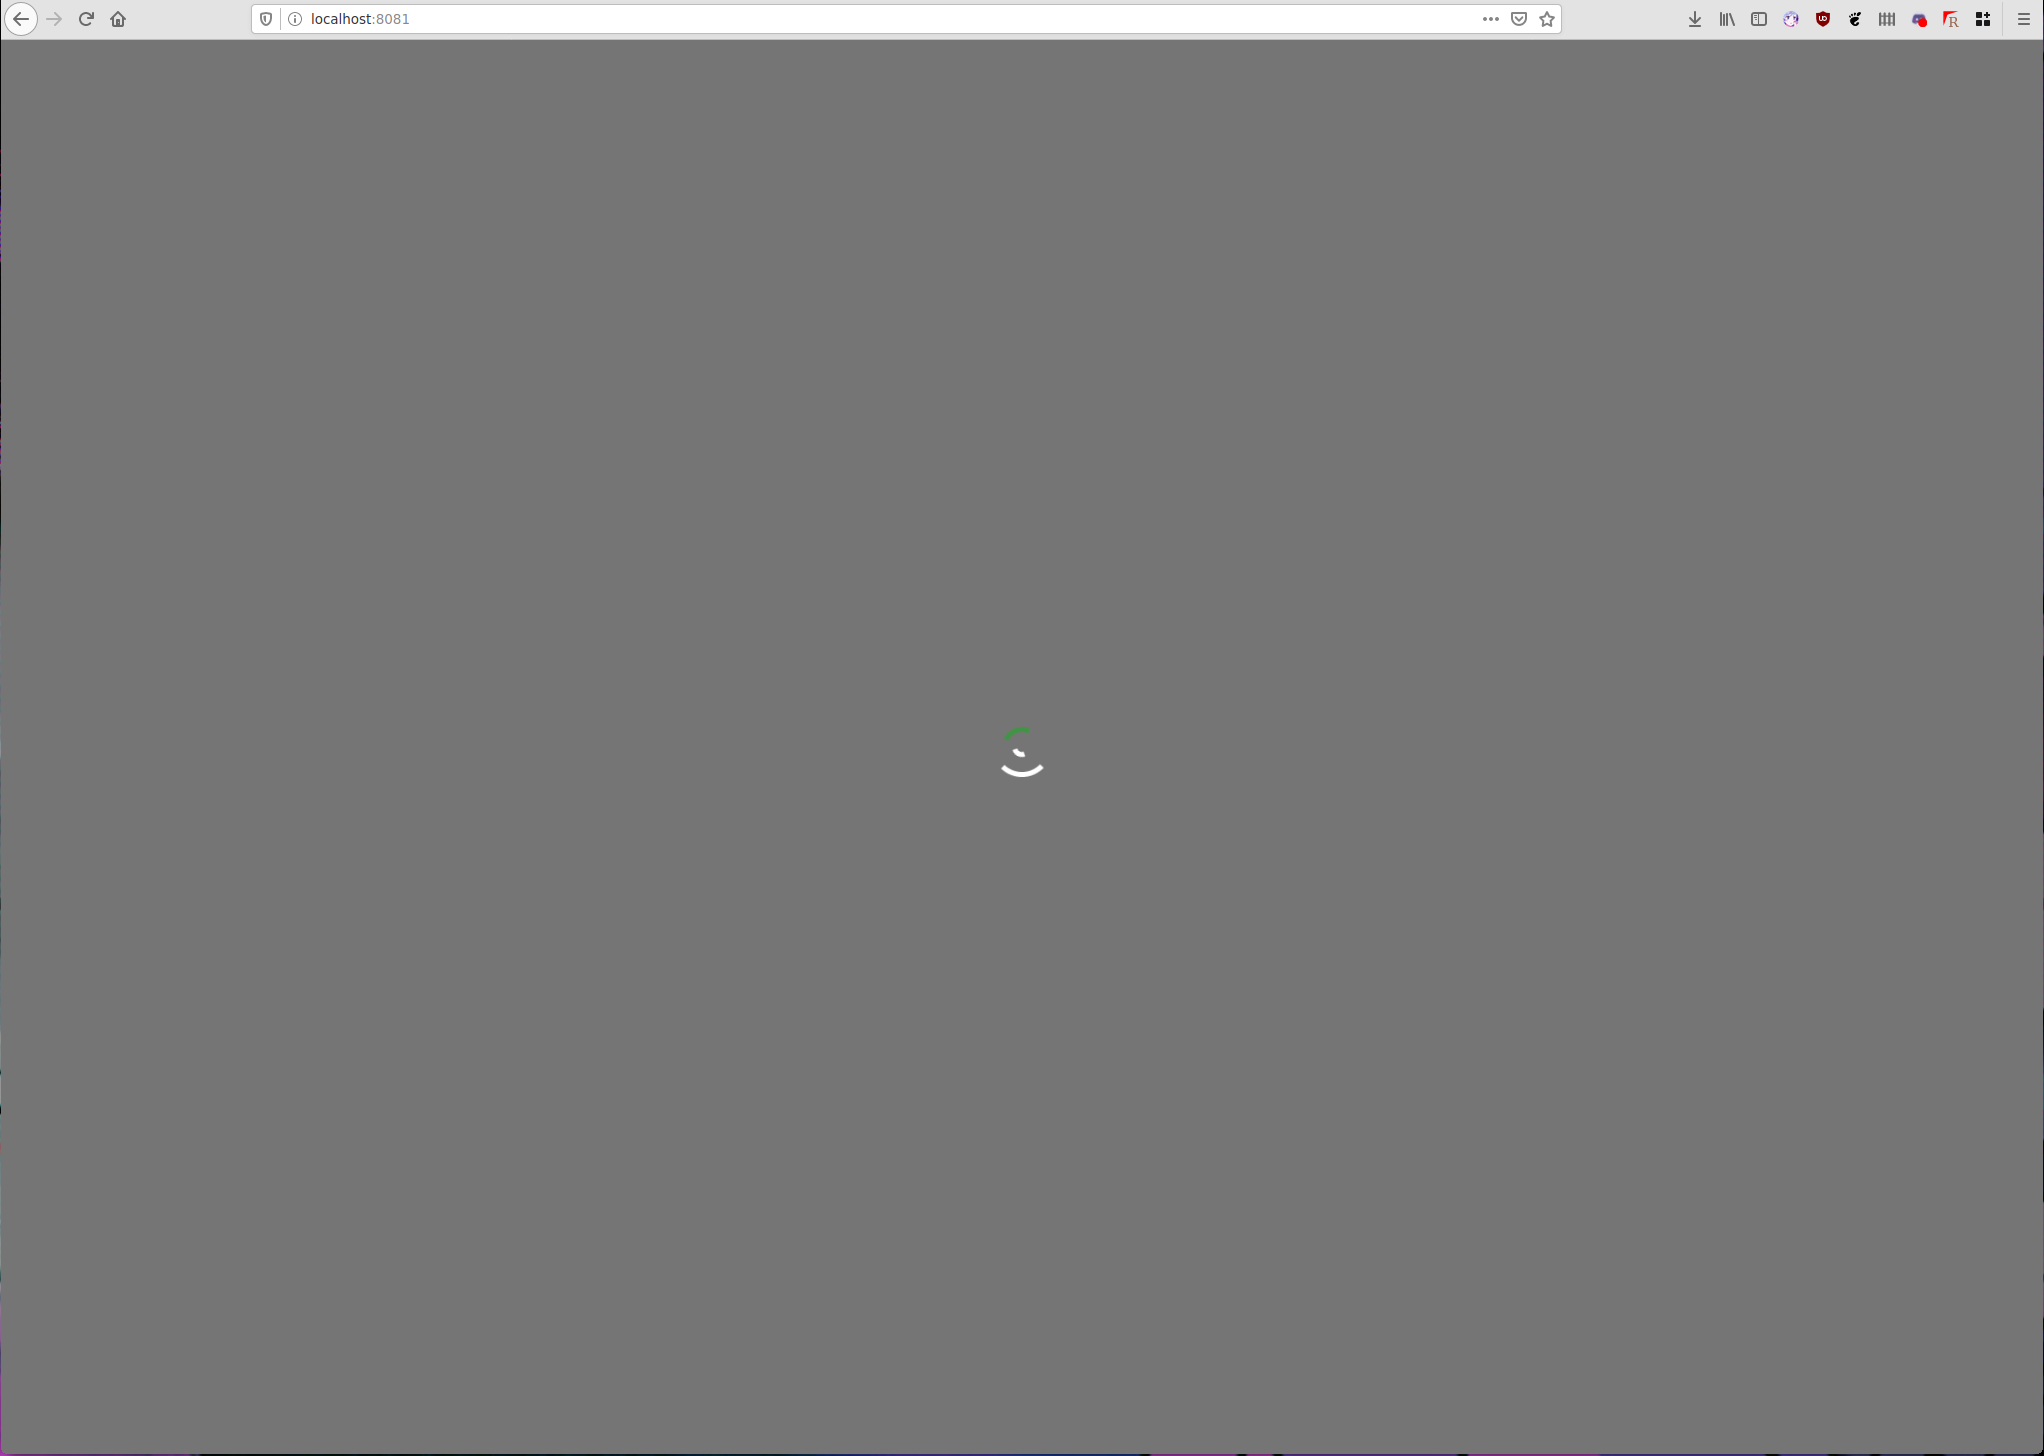
\includegraphics[width=.9\textwidth]{fragments/thinkno.png}
    \caption{ Pantalla de carga de think agro}
    \label{asd}
\end{figure}

Este hecho, hace que las pruebas de análisis dinámico y pentesting queden invalidados para el examen de esta aplicación. Lamentablemente, esta es la única aplicación de mi autoría desarrollada dentro de mi período de estudiante el cual cumple con los requisitos para ser evaluada. Por otro lado, para poder montar una versión de producción, es necesario contar con una subscripción de AWS con servicios de Route53, RDS, EC2, ElasticBeanstalk, CertificateManager, WAF y VPC activas, las cuales no es posible obtener dentro del marco de este trabajo.

Sin embargo, esto tampoco cambiaría el panorama ya que para efectos concretos, todo el tráfico es manejado por medio de un balanceador de carga, el cual impide la conexión a otros servicios desde fuera de la red interna. Por último, todas las conexiones entre los sistemas previamente existentes son realizadas desde la plataforma desarrollada y no hacia esta, lo cual impide que un sistema externo esté enviando información, ergo, no tiene otros puntos de entrada.

Una de las ventajas que ofrece tener todo en contenedores (independiente de lo presentado anteriormente) es una separación dura de los privilegios de ejecución de cada programa. Para esto, como descisión de despliegue se utiliza la premisa del mínimo permiso disponible y de contenedor atómico. Esto quiere decir que un contenedor solo tiene los permisos mínimos para funcionar, los accesos minimos disponibles. Adicionalmente, en caso de comportamiento anormal, este es automáticamente reiniciado y su contenido transiente eliminado. 

Esto evita que un payload pueda quedar viviendo por un tiempo prolongado, además por parte del balanceador de carga, como la aplicación es stateless y no tiene preferencia de alocación por cliente, se vuelve imposible ejecutar una secuencia seguida de comandos sobre una misma máquina. Esto fue decidido así para poder ofrecer una alternativa de bajo costo a la seguridad en la ejecución.

Por último, en caso de que un contenedor esté comprometido, este no es capaz de alcanzar con sus privilegios a otro contenedor del mismo tipo por estar aislado, y tampoco es capaz de alcancar otros elementos de red por medio de otros procesos.

Estos fueron los argumentos que motivaron el despliegue sobre contenedores y el desarrollo de una aplicación stateless por sobre una implementación monolítica stateful.